\chapter{Il package di grafica}\label{chap:gui_package}
\begin{figure}[t]
 \centering
 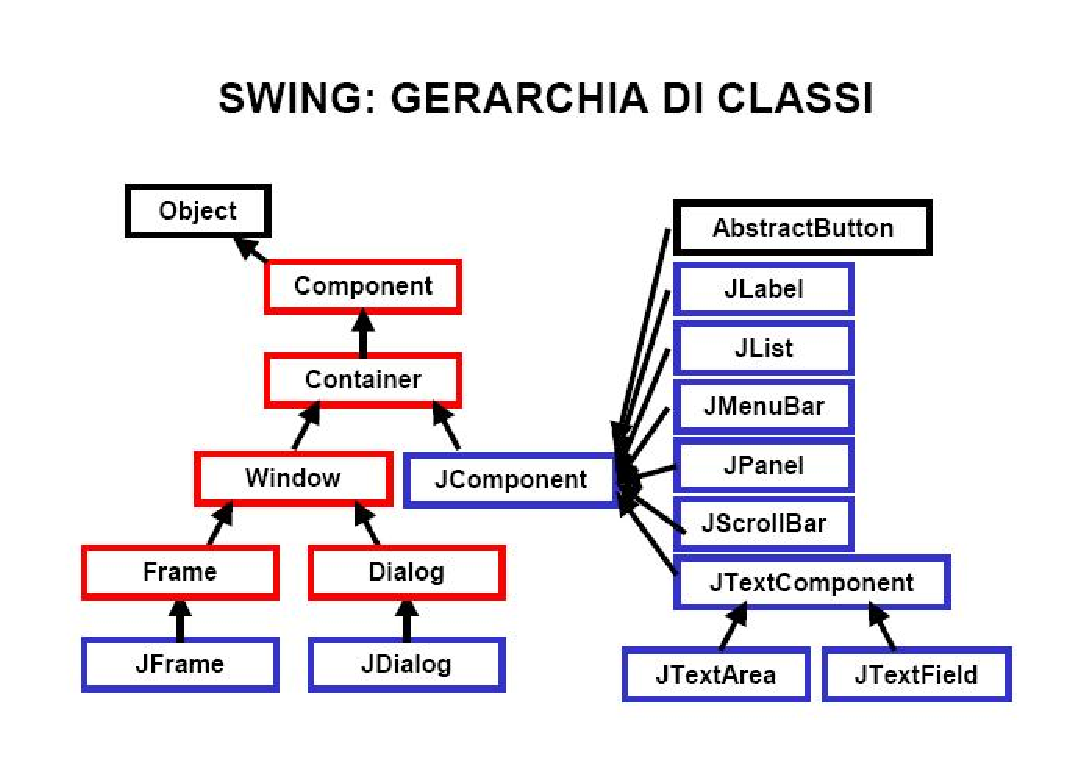
\includegraphics[width=350px,height=175px,bb=14 14 518 368]{images/swing_diagram.eps}
 % swing_diagram.eps: 0x0 pixel, 300dpi, 0.00x0.00 cm, bb=14 14 518 368
 \caption{La grafica con le librerie Swing.}
 \label{fig:swing_diagram}
\end{figure}

La parte grafica del MiniKazaa è stata implementata con la grafica che mette a disposizione il linguaggio Java e con l' ausilio dello strumento di programmazione NetBeans.
Nella parte che segue andiamo a vedere un pochino più di preciso cosa abbiamo usato per creare le interfaccie.

\section{Il campo di testo}
Il JTextField è un componente "campo di testo", usabile per scrivere e visualizzare una riga di testo.
Il campo di testo può essere editabile o no, il testo al suo interno è accessibile con getText() e modificabile con setText().
Ogni volta che il testo in esso contenuto cambia si genera un DocumentEvent nel documento che contiene il campo di testo.
Se invece è sufficiente registrare i cambiamenti solo quando si
preme INVIO, basta gestire semplicemente l' ActionEvent.

\section{I bottoni}
Quando viene premuto, un bottone genera un evento di classe ActionEvent.
Questo evento viene inviato dal sistema allo specifico ascoltatore degli eventi per quel bottone.
L'ascoltatore degli eventi deve implementare l' interfaccia ActionListener:
\begin{itemize}
\item può essere un oggetto di un'altra classe al di fuori del
pannello;
\item .. o può essere anche il pannello stesso nel quale (this).
\end{itemize}
Tale ascoltatore degli eventi deve implementare il metodo definito nella interfaccia actionListener void actionPerformed(ActionEvent ev);
che gestisce l'evento, nel senso che reagisce all'evento con opportune azioni.

\section{Gestore degli eventi}
Una volta generato l’oggetto evento, questo viene inviato ad un oggetto ascoltatore degli eventi (event listener).
L’event listener deve essere definito e creato da noi e deve essere associato al componente attivo, cosicché quando si genera un evento, la JVM sappia a chi inviare l’oggetto evento.
L’event listener gestisce l’evento mediante un opportuno metodo, che non è altro che l’implementazione di un particolare metodo di un’interfaccia associata a tali tipi
di eventi.


\section{Le tabelle di Java}
Una tabella è un componente che visualizza righe e colonne di dati. È possibile trascinare il cursore sui bordi delle colonne per ridimensionarle; è anche possibile trascinare una colonna in una nuova posizione. Le tabelle sono implementate dalla classe JTable.
Uno dei suoi costruttori è mostrato di seguito:
JTable(Object dati[][],Object intCol[])
dove dati è un array bidimensionale delle informazione da presentare e intCol è un array
monodimensionale con le intestazione delle colonne.
Ecco i passi per utilizzare una tabella in un frame:
\begin{itemize}
\item Creare un oggetto JTable
\item Creare un oggetto JScrollPane dove l'argomento del costruttore specifica la JTable appena creata. In questo modo la tabella verrà aggiunta al pannello
\item Aggiungere il pannello di scorrimento al pannello dei contenuti del JFrame (per intendere quello ottenuto tramite il metodo getContentPane()della classe)
\end{itemize}
Un JScrollPane è un pannello di scorrimento che presenta un'area rettangolare nella quale si può vedere un componente. Se il componente ha dimensione maggiore del pannello vengono fornite barre di scorrimento orizzontali e/o verticali.

